\documentclass[11pt,a4paper,oneside]{article}
\special{papersize=210mm,297mm}
\usepackage[left=2cm,text={17cm, 24cm},top=3cm]{geometry}
\usepackage{times}
\usepackage[utf8x]{inputenc} 
\usepackage[czech]{babel}
\usepackage[IL2]{fontenc}
\usepackage{cprotect}
\usepackage{tabu}
\usepackage{multirow}
\usepackage{graphics}
\usepackage{picture}
\usepackage{float}
\usepackage{amsmath}
\usepackage{amssymb}
\usepackage{amsthm}
\usepackage[linesnumbered,ruled,vlined]{algorithm2e}
\usepackage{epsfig}

\SetAlgorithmName{Algoritmus}{algoritmus}

\begin{document}

\begin{titlepage}
\begin{center}

{\Huge\textsc{{Vysoké učení technické v~Brně}}}\\
\bigskip
{\huge\textsc{{Fakulta informačních technologií}}}\\
\vspace{\stretch{0.382}}
{\LARGE{Typografie a publikování\,--\,3. projekt}}\\
\medskip
{\Huge{Tabulky a obrázky}}
\vspace{\stretch{0.618}}
\end{center}		
\Large{5. dubna 2015 \hfill Jan Ondruch}
\end{titlepage}

	\section{Úvodní strana}
	
	Název práce umístěte do zlatého řezu a~nezapomeňte uvést dnešní datum a~vaše jméno a~příjmení.
		
	\section{Tabulky}
	
	Pro sázení tabulek můžeme použít buď prostředí\texttt{ tabbing } nebo prostředí\texttt{ tabular}.
	
	\cprotect\subsection{Prostředí\texttt{ tabbing}} 
	
	Při použití\texttt{ tabbing } vypadá tabulka následovně:

 	\begin{tabbing}
    		Vodní melouny ~~~~\= 35,-- ~~~~\= 1 kus \kill 
	    \bfseries Ovoce \>
	    \bfseries Cena \>
    		\bfseries Množství \\
    		Jablka \> 25,90 \> 3 kg\\
    		Hrušky \> 27,40 \> 2,5 kg\\
		Vodní melouny \> 35,-- \> 1 kus
	\end{tabbing} \medskip
		
\noindent Toto prostředí se dá také použít pro sázení algoritmů, ovšem vhodnější je použít prostředí\texttt{ algorithm } nebo\texttt{ algorithm2e }(viz sekce \ref{sek3}). 

	\cprotect\subsection{Prostředí\texttt{ tabular}} 	

	Další možnost, jak vytvořit tabulku, je použít prostředí\texttt{ tabular}. Tabulky pak budou vypadat takto \footnote{Kdyby byl problem s\texttt{ cline, }zkuste se podívat třeba sem: http://www.abclinuxu.cz/tex/poradna/show/325037.}:
	\medskip	
	
	\begin{table}[H]
	\centering
	\catcode`\-=12
		\begin{tabular}{|c|c|c|}
		\hline
		\multicolumn{1}{|c|}{\textbf{}} & \multicolumn{2}{c|}{\textbf{Cena}} \\ \cline{2-3} 
		\textbf{Měna} & \textbf{nákup} & \textbf{prodej} \\ \hline
			EUR & 27,34 & 27,42 \\
			GBP & 33,09 & 33,21 \\
			USD & 19,87 & 19,95 \\ \hline
		\end{tabular}
	\caption{Tabulka kurzů k~dnešnímu dni}
	\label{fig:tab1}
	\end{table}

	\bigskip

	\begin{table}[h]
	\catcode`\-=12
	\centering
	\begin{tabular}{|c|c|}
	\hline
	$A$ & $\neg{A}$ \\ \hline
	\textbf{P} & N \\ \hline
	\textbf{O} & O~\\ \hline
	\textbf{X} & X \\ \hline
	\textbf{N} & P \\ \hline
	\end{tabular}
	\begin{tabular}{|c|c|c|c|c|c|}
	\hline
	\multicolumn{2}{|c|}{\multirow{2}{*}{A $\land$ B}} & \multicolumn{4}{c|}{$B$} \\ \cline{3-6} 
	\multicolumn{2}{|c|}{} & \textbf{P} & \textbf{O} & \textbf{X} & \textbf{N} \\ \hline
	\multirow{4}{*}{A} & \textbf{P} & P & O~& X & N \\ \cline{2-6} 
	 & \textbf{O} & O~& O~& N & N \\ \cline{2-6} 
	 & \textbf{X} & X & N & X & N \\ \cline{2-6} 
	 & \textbf{N} & N & N & N & N \\ \hline
	\end{tabular}
	\begin{tabular}{|c|c|c|c|c|c|}
	\hline
	\multicolumn{2}{|c|}{\multirow{2}{*}{A $\lor$ B}} & \multicolumn{4}{c|}{$B$} \\ \cline{3-6} 
	\multicolumn{2}{|c|}{} & \textbf{P} & \textbf{O} & \textbf{X} & \textbf{N} \\ \hline
	\multirow{4}{*}{A} & \textbf{P} & P & P & P & P \\ \cline{2-6} 
	 & \textbf{O} & P & O~& P & O~\\ \cline{2-6} 
	 & \textbf{X} & P & P & X & X \\ \cline{2-6} 
	 & \textbf{N} & P & O~& X & N \\ \hline
	\end{tabular}
	\begin{tabular}{|c|c|c|c|c|c|}
	\hline
	\multicolumn{2}{|c|}{\multirow{2}{*}{A $\rightarrow$ B}} & \multicolumn{4}{c|}{$B$} \\ \cline{3-6} 
	\multicolumn{2}{|c|}{} & \textbf{P} & \textbf{O} & \textbf{X} & \textbf{N} \\ \hline
	\multirow{4}{*}{A} & \textbf{P} & P & O~& X & N \\ \cline{2-6} 
	 & \textbf{O} & P & O~& P & O~\\ \cline{2-6} 
	 & \textbf{X} & P & P & X & X \\ \cline{2-6} 
	 & \textbf{N} & P & P & P & N \\ \hline
	\end{tabular}
	\caption{Protože Kleeneho trojhodnotová logika už je "zastaralá", uvádíme si zde příklad čtyřhodnotové logiky }
	\label{fig:tab2}
	\end{table}
	
	\pagebreak

\newpage
	\section{Algoritmy}\label{sek3}
	
	Pokud budeme chtít vysázet algoritmus, můžeme použít prostředí\texttt{ algorithm\footnote{Pro\,nápovědu,\,jak\,zacházet\,s~prostředím\texttt{ algorithm, }můžeme\,zkusit\,tuhle\,stránku:\\ 			http://ftp.cstug.cz/pub/tex/CTAN/macros/latex/contrib/algorithms/algorithms.pdf.} } nebo\texttt{ algorithm2e}\footnote{Pro\texttt{ algorithm2e }zase tuhle: 											http://ftp.cstug.cz/pub/tex/CTAN/macros/latex/contrib/algorithm2e/algorithm2e.pdf.}.\\
	Příklad použití prostředí\texttt{ algorithm2e }viz Algoritmus \ref{algoritmus}.
	
\begin{algorithm}
  \SetAlgoNoLine
  \SetNlSkip{-1.20em}
  \SetNlSty{}{}{:}
  \SetKwInput{Input}{Input}
  \SetKwInOut{Output}{Output}
  \SetKwFor{For}{for}{do}{end\,for}
    \Input{$(X_{t-1},u_t,z_t)$}
    \Output{$X_t$} 
\Indp
  \BlankLine
  $\overline{X_t} = X_t = 0$ \BlankLine   
  \For{$k = 1$ to $M$}{   
  		$\;\:x_t^{[k]} = sample\_motion\_model(u_t, x_{t-1}^{[k]})$ \\
    		$\;\:\omega_t^{[k]} = measuremen\_model(z_t, x_{t}^{[k]}, m_{t-1}^{[k]})$ \\
    		$\;\:m_t^{[k]} = updated\_occupancy\_grid(z_t, x_{t}^{[k]}, m_{t-1}^{[k]})$ \\
    		$\;\:\overline{X_t} = \overline{X_t} + \langle x_x^{[m]},\omega_t^{[m]} \rangle $
  }
  \For{$k = 1$ to $M$}{   
     \hspace{0.4em}draw $i$ with probability $\approx \omega_t^{[i]}$ \\
     \hspace{0.4em}add $\langle x_x^{[k]},m_t^{[k]} \rangle$ to $X_t$
  }
  \Return{$X_t$}
        
\caption{\textsc{Fast}SLAM\label{algoritmus}}
\end{algorithm}
	
	\section{Obrázky}
	
	Do našich článků můžeme samozřejmě vkládat obrázky. Pokud je obrázkem fotografie, můžeme klidně použít bitmapový soubor. Pokud by to ale mělo být nějaké schéma nebo něco podobného, je dobrým zvykem takovýto obrázek vytvořit vektorově.	
	
	\begin{figure}[H]
  		\centering
		\scalebox{0.4}{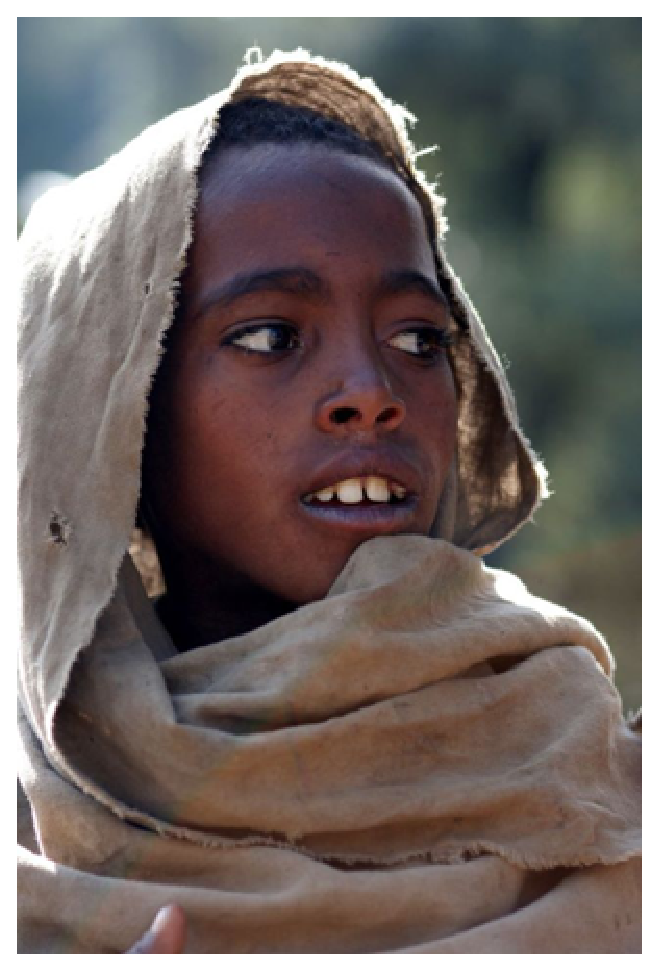
\includegraphics{etiopan.eps}
		\reflectbox{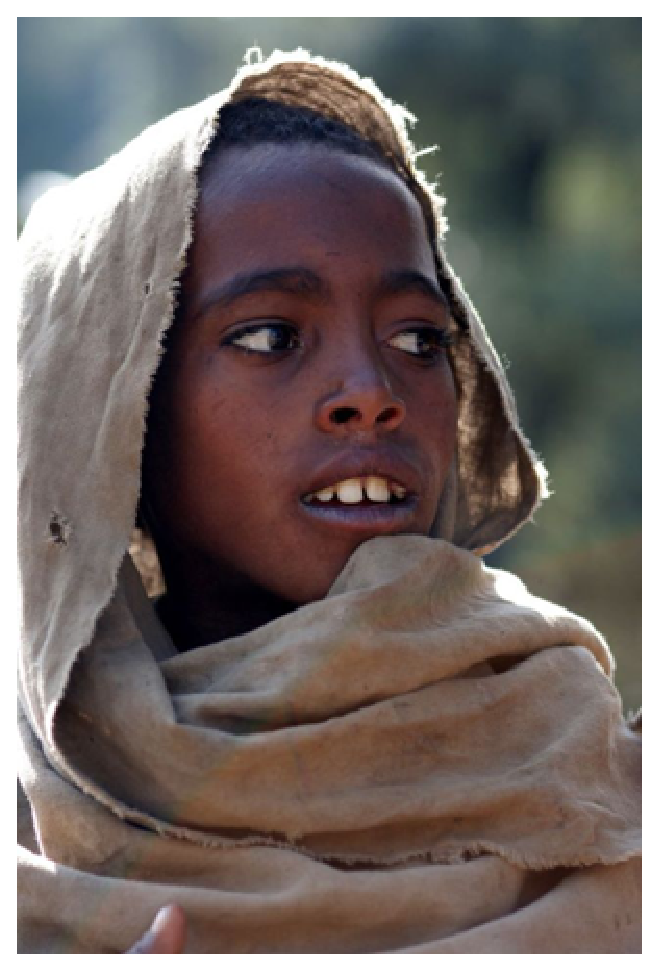
\includegraphics{etiopan.eps}} }
		\caption{Malý etiopánek a~jeho bratříček}
 		\label{fig:pic1}
	\end{figure}
	
	Rozdíl mezi vektorovým \dots	
	
	\begin{figure}[H]
  		\centering
		\scalebox{0.4}{
\includegraphics{oniisan.eps}}
		\caption{Vektorový obrázek}
 		\label{fig:pic2}
	\end{figure}
	
	\bigskip
	
	\noindent \dots a~bitmapovým obrázkem 
	
	\begin{figure}[H]
  		\centering
		\scalebox{0.6}{
\includegraphics{oniisan2.eps}}
		\caption{Bitmapový obrázek}
 		\label{fig:pic3}
	\end{figure}

	\bigskip
	
	\noindent se projeví při zvětšení.
	
	Odkazy (nejen ty) na obrázky \ref{fig:pic1}, \ref{fig:pic2}, \ref{fig:pic3}, na tabulky \ref{fig:tab1} a~\ref{fig:tab2} a~také algoritmus \ref{algoritmus} jsou udělány pomocí křižových odkazů. Pak je ovšem potřeba zdrojový soubor přeložit dvakrát.

Vektorové obárzky lze vytvořit i~přímo v~{\LaTeX}u, například pomocí prostředí\,\,\texttt{picture. }Všechny rozměry jsou uváděny v~mm.

\newpage

\begin{figure}
\begin{center}
	\setlength{\unitlength}{1.35mm}

\begin{picture}(115,158.5)


\put(0,0){\linethickness{1pt}\framebox(115,158.5){}}

  	\put(91,145){\makebox(15,14.5){\shortstack{Výška \\ mezery\,=\,14,5}}}
  		\put(88,151.25){\vector(0,-1){7.25}}
		\put(88,151.25){\vector(0,1){7.25}}
  
	\put(89,132){\makebox(15,14.5){\shortstack{Výška \\ mezery\,=\,10}}}
  		\put(88,139){\vector(0,1){5}}
  		\put(88,139){\vector(0,-1){5}}
  
  	\put(90,122){\makebox(15,14.5){\shortstack{Výška \\ hlavičky\,=\,10}}}
  		\put(88,129){\vector(0,1){5}}
  		\put(88,129){\vector(0,-1){5}}
  
  	\put(89,110){\makebox(15,14.5){\shortstack{Výška \\ mezery\,=\,14}}}
  		\put(88,117){\vector(0,-1){7}}
  		\put(88,117){\vector(0,1){7}}
  
  	\put(94,77.5){\linethickness{1pt}\framebox(15,10){\textbf{\shortstack{Okrajová\\ poznámka}}}}
  	
  	\put(92,88){\makebox(20,14.5){\shortstack{Šířka\\ boxu\,=\,15}}}
  		\put(102,91.5){\vector(-1,0){7.5}}
  		\put(102,91.5){\vector(1,0){7.5}}
  		
  	\put(87.5,97.5){\makebox(20,14.5){\shortstack{Mezera\,=\,9}}}
  		\put(90,91.5){\vector(-1,0){4.5}}
  		\put(94,103.5){\vector(-1,-3){4}}
  		\put(90,91.5){\vector(1,0){4.5}}
  
  	\put(87.5,57){\makebox(15,14.5){\shortstack{Výška\\ těla\,=\,75}}}
  		\put(88,72.5){\vector(0,-1){37.5}}
  		\put(88,72.5){\vector(0,1){37.5}}
  
  	\put(88,6){\makebox(15,14.5){\shortstack{Výška\\ paty\,=\,10}}}
  		\put(88,15){\vector(0,1){5}}
  		\put(88,15){\vector(0,-1){5}}
  
  	\put(89.5,19){\makebox(15,14.5){\shortstack{Výška\\ mezery\,=\,15}}}
  		\put(88,27.5){\vector(0,1){7.5}}
  		\put(88,27.5){\vector(0,-1){7.5}}

  	\put(53,3){\makebox(10,5){\shortstack{Šířka stránky = 115}}}
  		\put(57.5,3){\vector(1,0){57.5}}
  		\put(57.5,3){\vector(-1,0){57.5}}
  
  	\put(2.5,91.5){\makebox(10,5){\shortstack{Mezera = 15}}}
  		\put(7.5,91.5){\vector(-1,0){7.5}}
  		\put(7.5,91.5){\vector(1,0){7.5}}

  	\put(94,43){\makebox(15,14.5){\shortstack{Výška\\ stránky\,=\,158,5}}}
  		\put(102,55){\vector(1,1){10}}
  		\put(112,79.25){\vector(0,1){79.25}}
  		\put(112,79.25){\vector(0,-1){79.25}}

  	\multiput(15,151.5)(0,-10){16}{\line(0,1){7}}
  	\multiput(0,144)(10,0){11}{\line(1,0){7}}

  	\put(53,137){\makebox(10,5){\shortstack{Šířka boxu = 55}}}
  		\put(57.5,137){\vector(1,0){27.5}}
  		\put(57.5,137){\vector(-1,0){27.5}}
  	\put(30,124){\linethickness{1pt}\framebox(55,10){\textbf{Hlavička}}}

  	\put(30,35){\linethickness{1pt}\framebox(55,75){\textbf{Textové tělo}}}
  	\put(30.5,10){\linethickness{1pt}\framebox(55,10){\textbf{Pata}}}
  \end{picture}
\caption{Vektorový obrázek v~prostředí \texttt{picture}}
\end{center}
\end{figure}
	
\end{document}